% --------------------------------------------------------------
% This is all preamble stuff that you don't have to worry about.
% Head down to where it says "Start here"
% --------------------------------------------------------------

\documentclass[12pt]{article}

\usepackage[margin=1in]{geometry}
\usepackage{amsmath,amsthm,amssymb}
\usepackage{graphicx} %This allows to include eps figures
\usepackage{subcaption}
\usepackage[section]{placeins}
\usepackage{layout}
\usepackage{etoolbox}
\usepackage{mathabx}
% This is to include code
\usepackage{listings}
\usepackage{xcolor}
\definecolor{dkgreen}{rgb}{0,0.6,0}
\definecolor{gray}{rgb}{0.5,0.5,0.5}
\definecolor{mauve}{rgb}{0.58,0,0.82}
\lstdefinestyle{Python}{
    language        = Python,
    basicstyle      = \ttfamily,
    keywordstyle    = \color{blue},
    keywordstyle    = [2] \color{teal}, % just to check that it works
    stringstyle     = \color{green},
    commentstyle    = \color{red}\ttfamily
}

\newcommand{\N}{\mathbb{N}}
\newcommand{\Z}{\mathbb{Z}}

\newenvironment{theorem}[2][Theorem]{\begin{trivlist}
\item[\hskip \labelsep {\bfseries #1}\hskip \labelsep {\bfseries #2.}]}{\end{trivlist}}
\newenvironment{lemma}[2][Lemma]{\begin{trivlist}
\item[\hskip \labelsep {\bfseries #1}\hskip \labelsep {\bfseries #2.}]}{\end{trivlist}}
\newenvironment{exercise}[2][Exercise]{\begin{trivlist}
\item[\hskip \labelsep {\bfseries #1}\hskip \labelsep {\bfseries #2.}]}{\end{trivlist}}
\newenvironment{reflection}[2][Reflection]{\begin{trivlist}
\item[\hskip \labelsep {\bfseries #1}\hskip \labelsep {\bfseries #2.}]}{\end{trivlist}}
\newenvironment{proposition}[2][Proposition]{\begin{trivlist}
\item[\hskip \labelsep {\bfseries #1}\hskip \labelsep {\bfseries #2.}]}{\end{trivlist}}
\newenvironment{corollary}[2][Corollary]{\begin{trivlist}
\item[\hskip \labelsep {\bfseries #1}\hskip \labelsep {\bfseries #2.}]}{\end{trivlist}}

\begin{document}

% --------------------------------------------------------------
%                         Start here
% --------------------------------------------------------------

%\renewcommand{\qedsymbol}{\filledbox}

\title{Assignment 2}%replace X with the appropriate number
\author{Nalet Meinen\\ %replace with your name
Finite Element Analysis I
}

\maketitle

\tableofcontents
\pagebreak
\section{Introduction}
In this assignment three main methods will be analyzed: linear filtering, edge and corner detection. All of those things
base on the same algorithms or functions witch have to be implemented.

\section{Methods}

\subsection{Linear Filtering}
\begin{figure}[!htb]
  \centering
  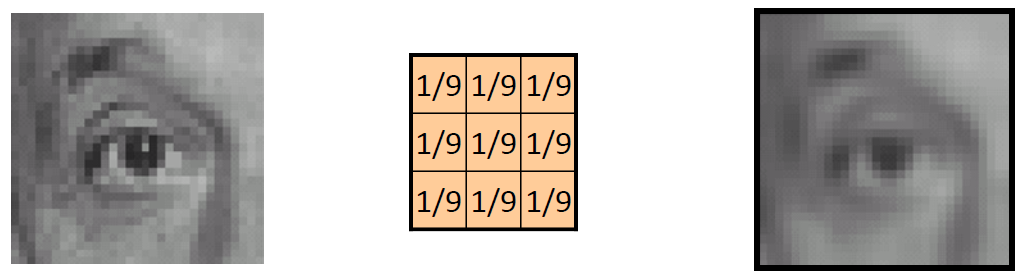
\includegraphics[width=0.7\textwidth]{pics/linear_filtering}
  \caption{Example of a boxfilter}
  \label{fig:linear_filtering}
\end{figure}

Linear filterings belongs to the group of neighbour analysis \cite{comp_intro}. As the 
name neighbour analysis says, the goal is to choose a pixel and analyse its neighbours.
With the information of the neighbours and depending on our processing strategy it is 
made possible to modify or enhance images. Applied cases can be smoothing an image or even
face recognition. Fig. \ref{fig:linear_filtering} shows a boxfilter using a $1/9$ of all
the pixels of the neighbours and the center giving us a blurred image.

\subsection{Finding Edges}
\begin{figure}[!htb]
  \centering
  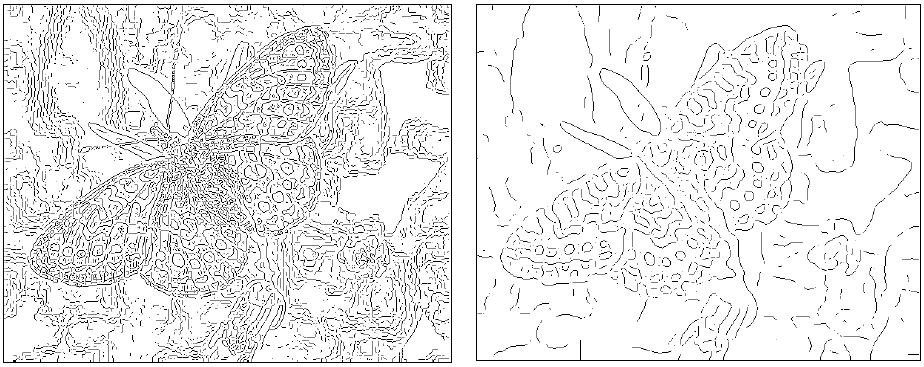
\includegraphics[width=0.7\textwidth]{pics/canny}
  \caption{Canny edge detection with (left) high threshold and (right) low threshold}
\end{figure}
Edges are boundary pixels which correspond to changes in gradients of physical changes
in object appearance. The most shapes in an image are consisting of edges. In Fig \ref{fig:canny}
a so called canny edge algorithm is applied. The high and low threshold determines the density of
edges we would like to have. Edge detection lies the fondation for basic shape detection in 
signal and image processing.

\subsection{Corner Detection}
\begin{figure}[!htb]
  \centering
  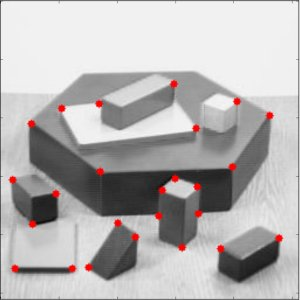
\includegraphics[width=0.3\textwidth]{pics/corner_detection}
  \caption{Canny edge detection with (left) high threshold and (right) low threshold}
  \label{fig:canny}
\end{figure}
Fig. \ref{fig:canny} shows us a image with many corners. The red dots are the corner detected.
Using the two methods from above, one can achive such an image output. From a pratical perspective
corner detection can be used to detect distortion from a perspective in an image or in medical
appliences for calibrating instrumens in the OR\footnote{Operation Room}
\pagebreak
\section{Results and Discussion}

\subsection{Linear Filtering}

\subsubsection{Boxfilter}
The boxfilter is a simple one liner. In the development phase the boxfilter was validated with the
debug function of the IDE.
\subsubsection{2D Convolution}
The algorithm checks the dimensions first before proceeding and if nessecary, reshaping. After preparing the output,
a full convolution is made.

\subsubsection{Applied Boxfilter}
\begin{figure}[!htb]
  \centering
  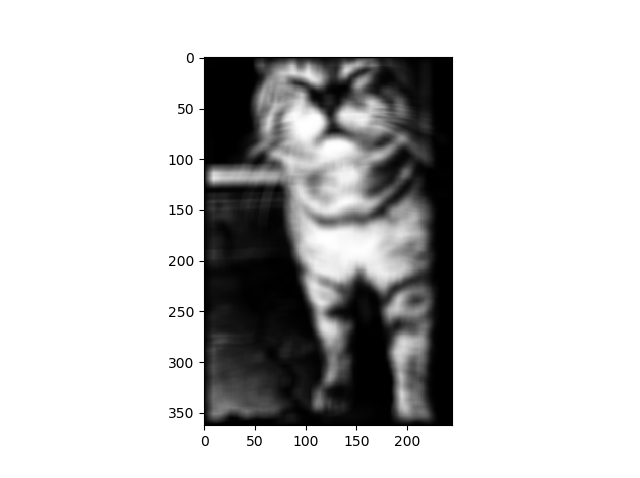
\includegraphics[width=0.8\textwidth]{pics/1_3_s}
  \caption{Applied box filter}
\end{figure}
Result of the applied box filter

\subsubsection{1D Gaussian Filter}
As described in the task, we using checks for making the filter odd. For performance reasons,
the numpy library with array multiplications and division is used.

\subsubsection{2D Gaussian Filter}
\begin{figure}[!htb]
  \centering
  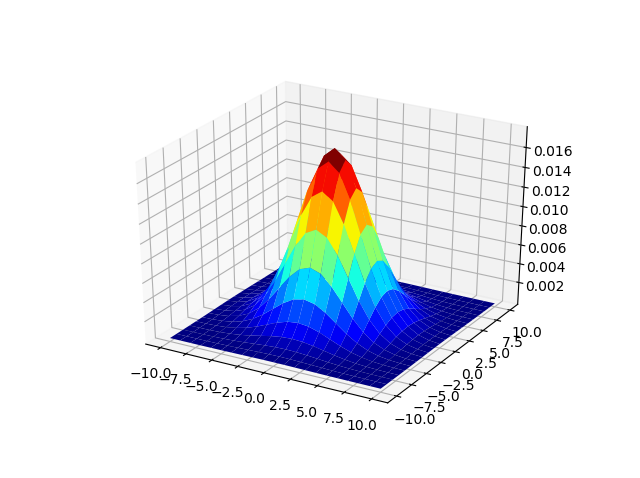
\includegraphics[width=0.7\textwidth]{pics/1_5_s}
  \caption{Gaussian kernel in 3D space}
\end{figure}
Result of the Gaussian 1D and the $myconf$ function.

\subsubsection{Applied 2D Gaussian Filter}
\FloatBarrier
\begin{figure}[!htb]
  \centering
  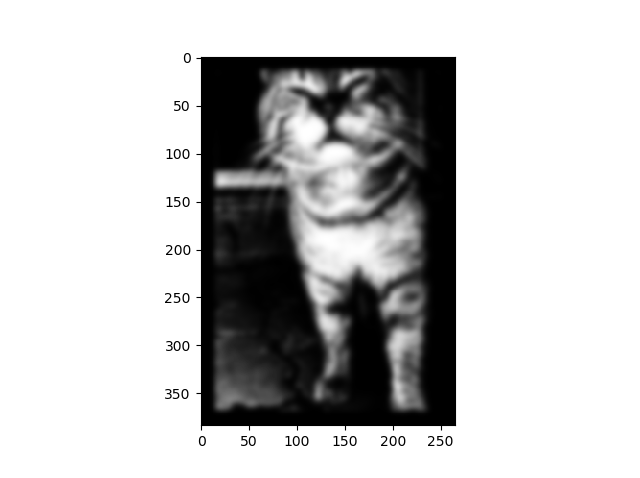
\includegraphics[width=0.6\textwidth]{pics/1_6_s}
  \caption{Result of the gaussian on an image}
\end{figure}
Applied result of our functions.
\pagebreak
\FloatBarrier
\subsubsection{Convolution with a 2D Gaussien Filter}
This text is also in the code. \newline
For each pixel the operations for convolution are n*n, n equals the size, width,
and height. Usually, this can be made faster with performing a 1d convolution in
both directions, horizontal and vertical, resulting in 2*n operations for a pixel.
Convolutions can then be split up. Looking at SVD, with one non-zero
value the separations in 1d can be made.

\subsubsection{Computation Time}
\begin{figure}[!htb]
  \centering
  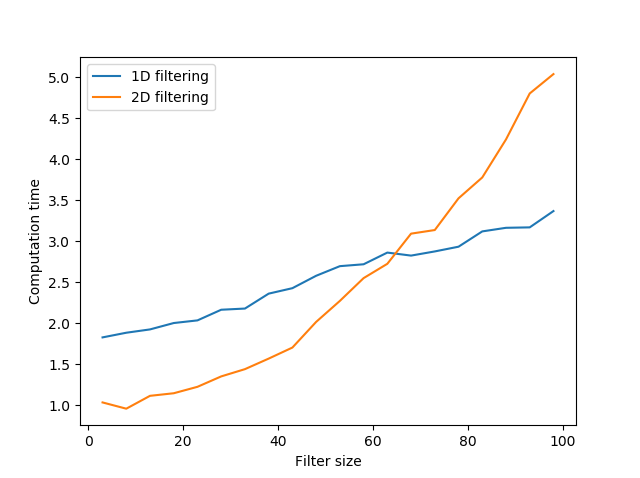
\includegraphics[width=0.8\textwidth]{pics/1_8_s}
  \caption{Compairson of 1D and 2D Gaus}
\end{figure}
We see that the slop of 2D filtering curve is much steeper, because of the factor 2 of
the number of dimensions to be calculated.
\newpage
\subsection{Finding Edges}
The needed functions are imported via the import statement of python. Measurement has been made,
that the code of ex1 does not run on the import. These could be made with $if \_\_name\_\_ == '\_\_main\_\_':$

\subsubsection{Derivative Operator}
Simple implementation of the derivative operator like proposed: $[1, 0, -1]$
\subsubsection{Edge Magnitude}
\begin{figure}[!htb]
  \centering
  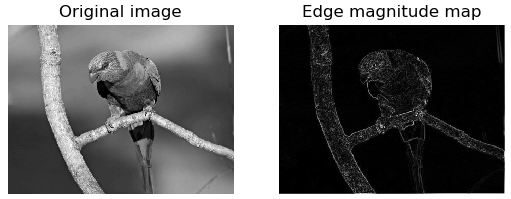
\includegraphics[width=0.8\textwidth]{pics/2_2_s}
  \caption{Edge Magnitude}
\end{figure}
Result of Edge Magnitude

\newpage
\subsubsection{Edge Images of Particular Directions}
\begin{figure}[!htb]
  \centering
  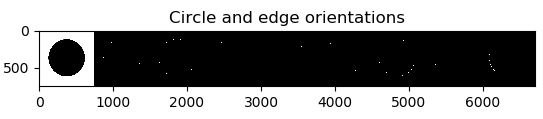
\includegraphics[width=0.8\textwidth]{pics/2_3_s}
  \caption{Result of a Circle}
\end{figure}
\begin{figure}[!htb]
  \centering
  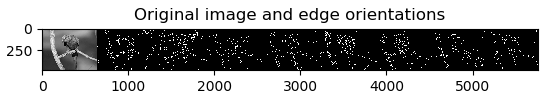
\includegraphics[width=0.8\textwidth]{pics/2_3_s2}
  \caption{Result of an image}
\end{figure}
Results of the edge orientations in both images.

\subsubsection{Edge Non-Max Suppression}
\begin{figure}[!htb]
  \centering
  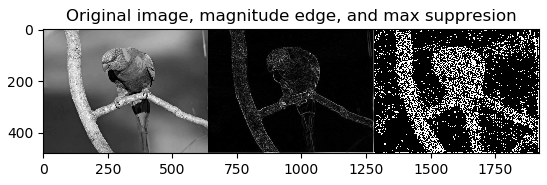
\includegraphics[width=0.8\textwidth]{pics/2_4_s}
  \caption{Image output of ex 2.4}
\end{figure}
Result of the polot of the original image, maginitude edge and the max suppression

\newpage
\subsubsection{Canny Edge}
\begin{figure}[!htb]
  \centering
  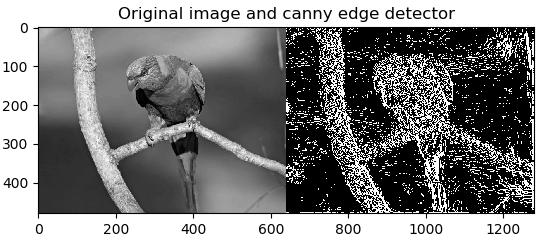
\includegraphics[width=0.8\textwidth]{pics/2_5_s}
  \caption{Result canny edge}
\end{figure}
Here a first result of the canny edge detector, the result. A different approch was taken as in max suppression.
The idea was a simpler code, but the result is not quite satifying, as the threshold are not working as expected.

\newpage
\subsection{Corner Detection}

\subsubsection{Harris Corner}
The Harris Corner algorithm was implemented accourding to the steps from the slides ina
the lectures.
\subsubsection{Evaluation of Harris Corner}
\begin{figure}[!htb]
  \centering
  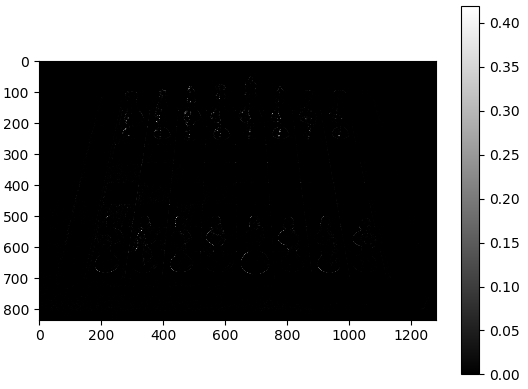
\includegraphics[width=0.5\textwidth]{pics/3_2_s}
  \caption{Result Harris Corner}
\end{figure}
Plot from python program. The plot is quite dark but the result is good, as you can see later.

\subsubsection{Rotation}
\begin{figure}[!htb]
  \centering
  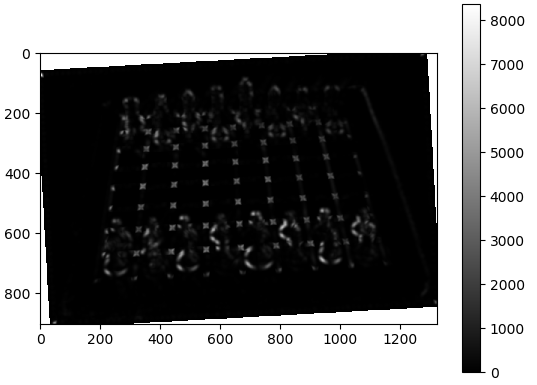
\includegraphics[width=0.5\textwidth]{pics/3_3_s}
  \caption{Result Harris Corner after the rotation}
\end{figure}
Plot from python program after rotation.

\newpage
\subsubsection{Factor of Halv}
\begin{figure}[!htb]
  \centering
  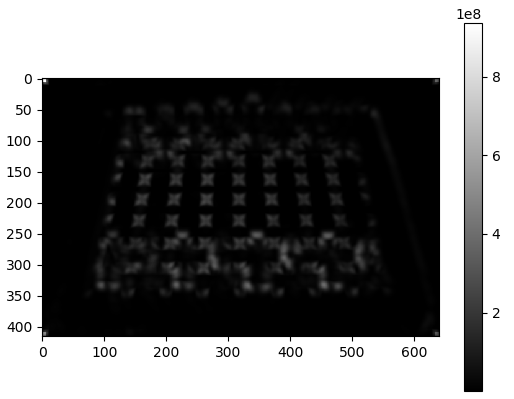
\includegraphics[width=0.5\textwidth]{pics/3_4_s}
  \caption{Result canny edge}
\end{figure}
Plot from python program after scaling. The edges become more visible, larger because auf thebibliography
new resolution.

\subsubsection{Properties of Harris Corner}
The Harris Corner is a region, where a gradient goes in diferent directions. But these regions are difficult to
differentiate from edges with a high gradient in only one direction. It is invariant to scaling (as seen above)
because the structure matrix can be used for diagonal directions, better as from other gradients in x and y directions.

\newpage
\subsection{Conclusion}
In this assigment, many different approches for filtering have been examined. It is interesting that all of those appliences 
have same origins, in our case, same methods that can be reused. Compared to the default implementation of numpy or cv2, or 
implementation is quite not optimized. During the development stage, compairsion with the library was made. In the last exercise
even the implementation of a library was used. Such basic function, must be robust and performant. So it is important from a 
mathematical or computer science perspective to be as accurate as possible, regarding to the use in medical appliances.


\begin{thebibliography}{1}
  \bibitem{comp_intro} 
  Alasdair McAndrew
  \\\textit{A Computational Introduction to Digital Image Processing (2015)}. (English)  

  \bibitem{py_tutorials} 
  OpenCV Python Tutorials
  \\\textit{https://opencv-python-tutroals.readthedocs.io (2019)}. (English)  
\end{thebibliography}


\end{document}
